\section{Theorie}

\subsection{Der Aufbau der Geiger-Müller-Zählrohrs}
\begin{flushleft}
    Das Geiger-Müller-Zählrohr ist ein Zählrohr, welches aus einem Zylinderförmigen Mantel mit einem Draht in der Mitte besteht.
    Auf diesen Draht, welcher von einem Gasgemisch, bestehend aus Agon und Ethylalkohol, kann eine Betriebsspannung gelegt werden, wodurch eine Potentialdifferenz zwischen Mantel und Draht entsteht.
    Zu sehen ist so eine Geiger-Müller-Zählrohr in Abbildung \ref{Abbildung1}.
    Verwendet wird dieses um ionisierende Strahlung zu messen, da bei eintretender ionisierter Strahlung ein elektrischer Impuls abgegeben wird, der von einem Messgerät leicht gezählt werden kann.
    Das dabei entstehende elektrische Feld wird berechnet durch 
\end{flushleft}

\begin{equation}
    \text{E}(\text{r}) = \frac{\text{U}}{\text{r}\,\ln(\text{r}_{\text{k}}/\text{r}_{\text{a}})}\,. \notag
\end{equation}

\begin{figure}[H]
    \centering
    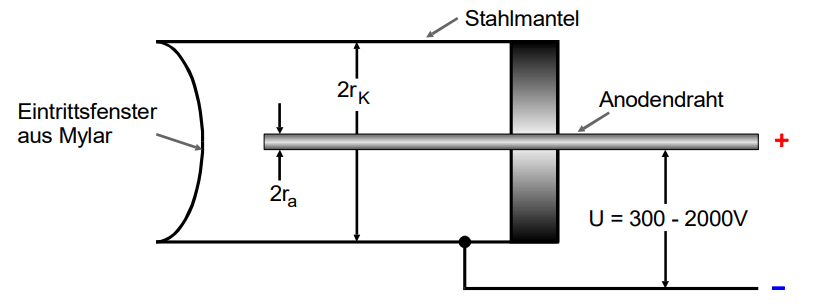
\includegraphics[height=40mm]{bilder/Ab1.png}
    \caption{Querschnitt durch ein Endfenster-Zählrohr \cite{a1}. \label{Abbildung1} }
\end{figure}

\subsection{Spannungsabhängiges Verhalten des Geiger-Müller-Zählrohrs}

\begin{flushleft}
    Bei Absorption eines geladenen Teilchens vom Rohr, wird dieses solange durch den Gasraum bewegt bis die Energie aufgrund von Ionisationskontakten aufgebraucht ist.
    Ebenfalls gibt es verschiedene Verhalten des Zählrohr die Spannungsabhängig sind. 
    Eingeteilt werden diese in fünf verschiedene Zonen, dessen Verlauf in Abbildung \ref{Abbildung2} bildlich dargestellt wird.
\end{flushleft}

\begin{flushleft}
    Die erste Zone ist die für kleine Betriebsspannungen, in welcher nur wenige Elektronen den Draht erreichen und die restlichen rekombinieren, bevor der Draht erreicht werden kann.
\end{flushleft}

\begin{flushleft}
    In der zweite Zone ist die Betriebsspannung schon höher, sodass sehr viele Elektronen den Draht erreichen können und ohne davor zu rekombinieren, was dazu führt, dass ein Ionisationsstrom erzeugt wird, der proportional zur Energie der ionisierenden Strahlung ist. 
\end{flushleft}

\begin{flushleft}
    In der dritten Zone ist die Spannung so hoch angelegt, dass die durch Ionisation entstandenen Elektronen so schnell durch das Elektrische Feld beschleunigt werden, dass sie andere Atome beim Zusammenstoßen mit ionisieren.
    Dabei kommt es zu einer Kettenreaktion welche auch als Townsend-Lawine bezeichnet wird.
\end{flushleft}

\begin{flushleft}
    Die vierte Zone ist die Zone, in welcher der Arbeitsbereich des Geiger-Müller-Zählrohr liegt.
    Durch die sehr hohen Spannungen, entstehen bei der Primärionisation in großer Zahl UV-Protonen, welche sich aufgrund der Ladungsneutralität senkrecht zum elektrischen Feld im Zählrohr ausbreiten.
    Dies sorgt für weitere Elektronenlawinen im gesamten Zählrohrvolumen und die daraus resultierenden elektrischen Impulse sind hinreichend groß, dass diese einfach mit einem Impulszähler gezählt werden können.
    Die letzte Zone ist die Entladungszone.
\end{flushleft}

\begin{figure}[H]
    \centering
    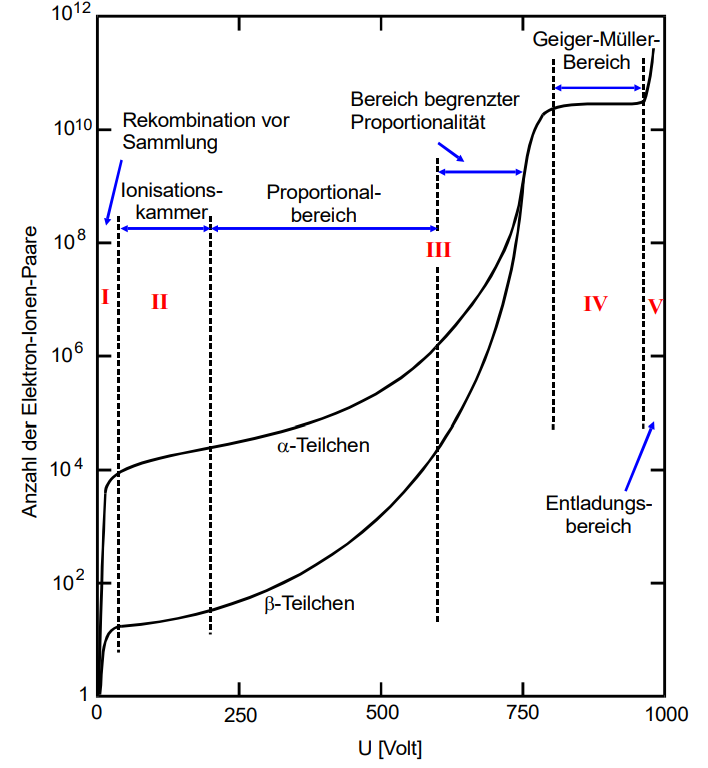
\includegraphics[height=140mm]{bilder/Ab2.png}
    \caption{Anzahl der erzeugten Elektron-Ionenpaare als Funktion der Spannung U bei einem Proportionalzählrohr (nach Kleinknecht, Detektoren für Teilchenstrahlen) \cite{a1}. \label{Abbildung2} }
\end{figure}

\subsection{Tot-, Erholungszeit und Nachentladungen}

\begin{flushleft}
    Eine radialsymmetrische Raumladung entsteht, da sich die positiven Ionen auf Grund ihrer größeren Masse langsamer zur Kathode bewegen. 
    Dies wird auch als Ionenschlauch bezeichnet. 
    Aus diesem Grund nimmt die Feldstärke für einen Zeitraum T sehr stark ab, sodass keine Stoßionisationen erfolgen können.
    Die Teilchen, die in der Zeit eintreffen können nicht registriert werden, dieser Zeitraum wird deshalb auch als Totzeit bezeichnet. 
    Es können wegen steigender Feldstärke weitere Lawinen ausgelöst werden. 
    Die zunächst registrierten Ladungsimpulse sind ein wenig schwächer, da das elektrische Feld erst kontinuierlich entstehen muss, wobei der Zeitraum, in dem dies stattfindet, als Erholungszeit bezeichnet wird. 
    Nebeneffekte bei dem Vorgang sind die Nachentladungen, da Elektronen aus dem Metall gelöst werden können, wenn die positiven Ionen aud dem Mantel treffen. 
    Diese lösen erneut Zählrohrentladungen aus. 
    In Abbildung \ref{Abbildung3} wird der beschriebenen Prozesse verbildlicht.
\end{flushleft}

\begin{figure}[H]
    \centering
    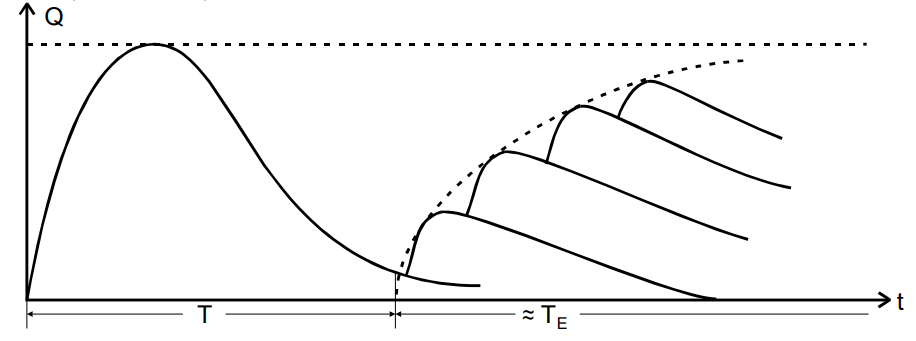
\includegraphics[height=50mm]{bilder/Ab3.png}
    \caption{Tot- und Erholungszeit eines Zählrohrs, dargestellt im Ladungs-Zeit-Diagramm \cite{a1}. \label{Abbildung3} }
\end{figure}

\subsection{Charakteristik des Zählrohrs}

\begin{flushleft}
    Der Arbeitsbereich eines Geiger-Müller-Zählrohr ist in Abbildung \ref{Abbildung4} zu sehen.
    Es fällt auf, dass zwischen der Spannung $\text{U}_{\text{E}}$, bei welcher der Auslösebereich eintritt, und dem Bereich wo die Dauerentladung eintritt, die Kurve einen linearen Verlauf annimmt.
    Dieser wird auch Plateau genannt, welches bei einem idealen Zählrohr nicht ansteigen würde, jedoch ist ein kleiner Anstieg aufgrund der Nachladung vorhanden.
\end{flushleft}

\begin{figure}[H]
    \centering
    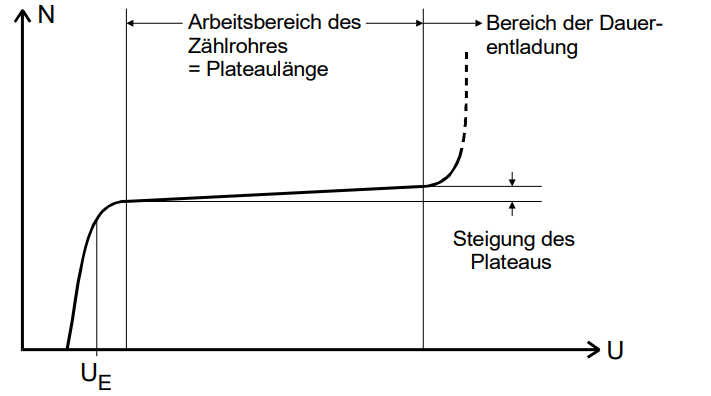
\includegraphics[height=80mm]{bilder/Ab4.png}
    \caption{Zählrohrcharakteristik \cite{a1}. \label{Abbildung4} }
\end{figure}

\subsection{Bestimmung der Totzeit mit der Zwei-Quellen-Methode}

\begin{flushleft}
    Durch die Totzeit kommt es dazu, dass die registrierte Impulsrate immer kleiner ist als die Anzahl absorbierter Teilchen
\end{flushleft}

\begin{equation}
    \text{N}_{\text{W}} = \frac{\text{Impulsrate}}{\text{Messzeit}} = \frac{\text{N}_{\text{r}}\,\text{t}}{(1 - \text{T}\,\text{N}_{\text{r}})\,\text{t}} = \frac{\text{N}_{\text{r}}}{1 - \text{T}\,\text{N}_{\text{r}} }\,. \label{1}
\end{equation}

\begin{align}
    \intertext{Würde keine Totzeit auftreten würde}
    \text{N}_{1+2} = \text{N}_{1} + \text{N}_{2}\,. \notag
    \intertext{gelten. 
    Jedoch wird beobachtet, dass}
    \text{N}_{1+2} < \text{N}_{1} + \text{N}_{2}\notag
    \intertext{gilt.
    Die Anzahl der in das Zählrohrvolumen eingedrungenen Teilchen wird mit der Gleichung (\ref{1}) berechnet, dadurch ergibt sich}
    \frac{\text{N}_{\text{1}}}{1 - \text{T}\,\text{N}_{\text{1}} }\,\notag
    \intertext{und}
    \frac{\text{N}_{\text{2}}}{1 - \text{T}\,\text{N}_{\text{2}} }\,.\notag
    \intertext{Da $\text{N}_{1+2} = \text{N}_{1} + \text{N}_{2}$ ist, folgt für die Totzeit Näherungsweise}
    \text{T} \approx \frac{\text{N}_{\text{1}} +\text{N}_{\text{2}} - \text{N}_{\text{1+2}}}{2\,\text{N}_{\text{1}}\,\text{N}_{\text{2}}}\,. \label{2}
\end{align}

\subsection{Messung der pro Teilchen vom Zählrohr freigesetzten Ladungsmenge}

\begin{align}
    \intertext{Mit Hilfe eines Strommessgerätes kann der mittlere Zählrohrstrom $\overline{\text{I}}$  gemessen werden, wodurch sich dann mit}
    \text{I} = \frac{\increment \text{Q}}{\increment \text{t}}\,\text{Z} \label{3}
    \intertext{die Ladungsmenge $\increment \text{Q}$ bestimmen lässt.} \notag
\end{align}